% Chapter: 03_transformer_features
% Included from lectures/main.tex

\section{Features in Language Models}

\begin{frame}{Features in Language Models}

\note{
\begin{itemize}
\item Doing MechInterp in language models is harder
\item We often do not have a privileged basis (the residual stream in a transformer is rotationally invariant)
\item It is not clear which directions are our features
\end{itemize}
}
\end{frame}

% mikolov2013: fig1 = Figure 2 (word vector diagram, left panel)
\begin{frame}{Features Represent Human-Understandable Concepts \cite{mikolov2013}}
\begin{center}

\includegraphics[height=0.55\textheight,keepaspectratio]{figures/mikolov2013/fig1.png}
\hspace{0.5em}

\includegraphics[height=0.55\textheight,keepaspectratio]{figures/mikolov2013/fig2.png}
\end{center}
\IfFileExists{03_transformer_features/figures/mikolov2013/fig1-caption.txt}{%
  \CatchFileDef{\captiontext}{03_transformer_features/figures/mikolov2013/fig1-caption.txt}{\endlinechar=-1}%
  {\tiny \captiontext}%
}{}

\note{
\begin{itemize}
\item We already saw this before we had LLMs, just for small RNNs that predict text
\item A particular direction encodes gender: we can extract that direction from a pair of opposite-gendered words
\item Adding it to one word brings us to its opposite-gendered counterpart
\end{itemize}
}
\end{frame}

\begin{frame}{}
\begin{center}
\Large How do we identify features in Transformers?
\end{center}

\note{
\begin{itemize}
\item How do we identify features in a transformer?
\item Gathering ideas from the audience, specifically people who have not heard much about MechInterp before
\end{itemize}
}
\end{frame}

\begin{frame}{Probes}
We can project activations at any point in the forward pass along any direction,
and thereby classify the input on a linear scale.

\note{
\begin{itemize}
\item We can just project the activations at any point in the forward pass along any direction, and thereby classify the input of the transformer on a linear scale
\item If the direction is a feature with some human-understandable meaning, we would expect it could classify inputs that have this meaning (a Spanish feature could classify Spanish text)
\item Or alternatively classify model cognition (a ``lying'' feature when the model decides to output a lie)
\end{itemize}
}
\end{frame}

% park2024: fig3 = Figure 4
\begin{frame}{Linear Probes Can Classify Text Properties \cite{park2024}}
\paperfig{figures/park2024/fig3.png}{03_transformer_features/figures/park2024/fig3-caption.txt}

\note{
\begin{itemize}
\item We can extract an English vs Spanish feature by embedding the words, subtracting them, and projecting on that direction
\item Doing that with a random word pair does not give you this distinction
\item This gives us evidence that human-understandable features exist in LLMs, and it seems somewhat easy to guess what they are
\item However, this just shows us we can extract a feature of the text
\item LLMs are not only cool because they model texts, they are also entities that reason and model the world
\item Can we extract these world-models from a transformer via finding the right feature directions?
\end{itemize}
}
\end{frame}

% nanda2023: fig0 = Figure 1 (board reconstruction), table0 = Table 1
\begin{frame}{Linear Probes Can Measure World Models \cite{nanda2023}}
\begin{columns}[c]
\begin{column}{0.55\textwidth}
\paperfig{figures/nanda2023/fig0.png}{03_transformer_features/figures/nanda2023/fig0-caption.txt}
\end{column}
\begin{column}{0.42\textwidth}
\paperfig{figures/nanda2023/table0.png}{03_transformer_features/figures/nanda2023/table0-caption.txt}
\end{column}
\end{columns}

\note{
\begin{itemize}
\item Othello-GPT: a transformer trained as a next token predictor on moves in an Othello game
\item They train linear probes on the residual stream to predict the state of each field on the board
\item One probe each for empty, ``mine'' (player whose turn it is), and ``yours'' (other player's pieces)
\item They could reconstruct the state of the game board with pretty high accuracy
\end{itemize}
}
\end{frame}

% nanda2023: fig1 = Figure 2 (intervention diagram), table1 = Table 2
\begin{frame}{Intervening on the World Model \cite{nanda2023}}
\begin{columns}[c]
\begin{column}{0.55\textwidth}
\paperfig{figures/nanda2023/fig1.png}{03_transformer_features/figures/nanda2023/fig1-caption.txt}
\end{column}
\begin{column}{0.42\textwidth}
\paperfig{figures/nanda2023/table1.png}{03_transformer_features/figures/nanda2023/table1-caption.txt}
\end{column}
\end{columns}

\note{
\begin{itemize}
\item Once they knew the direction, they could also add those directions in to change the model's beliefs about what piece is there
\item They did this by adding the direction encoding a particular game state in every layer of the residual stream
\item The model afterwards continued playing as if this change on the game board actually happened
\end{itemize}
}
\end{frame}

% li2024b: fig1 = Figure 2 (probe heatmap + KDE)
\begin{frame}{Probing LLMs \cite{li2024b}}
\paperfig{figures/li2024b/fig1.png}{03_transformer_features/figures/li2024b/fig1-caption.txt}

\note{
\begin{itemize}
\item We can of course also train probes on the activations of LLMs
\item Here we see probes trained on the O values of the attention heads
\item We see that some heads can separate the activations on true vs false statements
\item We even see that they separate quite well on the first principal components
\end{itemize}
}
\end{frame}

% li2024b: fig2 = Figure 3 (ITI sketch), table0 = Table 1
\begin{frame}{Adding in Truthfulness \cite{li2024b}}
\begin{columns}[c]
\begin{column}{0.5\textwidth}
\paperfig{figures/li2024b/fig2.png}{03_transformer_features/figures/li2024b/fig2-caption.txt}
\end{column}
\begin{column}{0.47\textwidth}
\paperfig{figures/li2024b/table0.png}{03_transformer_features/figures/li2024b/table0-caption.txt}
\end{column}
\end{columns}

\note{
\begin{itemize}
\item They could also use these directions, extracted from probes, to steer the model to be more truthful
\item Only adding in the top $k$ most predictive heads, with factor $\alpha$, both tuned hyperparameters
\item They can outperform finetuning, and help on top of few-shot prompting
\end{itemize}
}
\end{frame}

% panickssery2024: fig0 = Figure 1a (contrastive pair diagram)
\begin{frame}{Steering via Contrastive Features \cite{panickssery2024}}
\paperfig{figures/panickssery2024/fig0.png}{03_transformer_features/figures/panickssery2024/fig0-caption.txt}

\note{
\begin{itemize}
\item You don't even need probes to extract these features
\item Just taking the average of activation differences of a bunch of contrastive examples of some behaviour is enough
\item You can, within some bound, pretty much steer arbitrary concepts that way
\end{itemize}
}
\end{frame}

% panickssery2024: fig7 = Figure 4 (CAA effect on multiple-choice)
\begin{frame}{Effect of Contrastive Activation Addition \cite{panickssery2024}}
\paperfig{figures/panickssery2024/fig7.png}{03_transformer_features/figures/panickssery2024/fig7-caption.txt}

\note{
\begin{itemize}
\item You can, within some bound, pretty much steer arbitrary concepts that way
\end{itemize}
}
\end{frame}

\begin{frame}{Ablating Features \cite{arditi2024}}
\textbf{Activation addition:}
\[ x^{(l)\prime} \leftarrow x^{(l)} + r^{(l)} \]

\vspace{0.5em}
\textbf{Direction ablation:}
\[ x' \leftarrow x - \hat{r}\hat{r}^\top x \]

\vspace{0.5em}
\textbf{Weight orthogonalization:}
\[ W'_{\text{out}} \leftarrow W_{\text{out}} - \hat{r}\hat{r}^\top W_{\text{out}} \]

\vspace{0.3em}
{\small $r$: feature direction \quad $x$: activation \quad $W$: weight matrix}

\note{
\begin{itemize}
\item Once we have a feature, we can do more than just adding it somewhere to see what happens
\item We can also ablate it out, and make a model basically blind to that concept
\item We can also fold this projection into the weights: if we do that to all weights that write into the residual stream, we have basically made the model blind to a concept
\item If I just hand you the weights it is not easy for you to see I did anything with it
\end{itemize}
}
\end{frame}

% arditi2024: fig0 = Figure 1 (refusal ablation), fig1 = Figure 2 (activation addition)
\begin{frame}{Refusal Is Mediated by a Single Direction \cite{arditi2024}}
\begin{columns}[c]
\begin{column}{0.5\textwidth}
\paperfig{figures/arditi2024/fig0.png}{03_transformer_features/figures/arditi2024/fig0-caption.txt}
\end{column}
\begin{column}{0.47\textwidth}
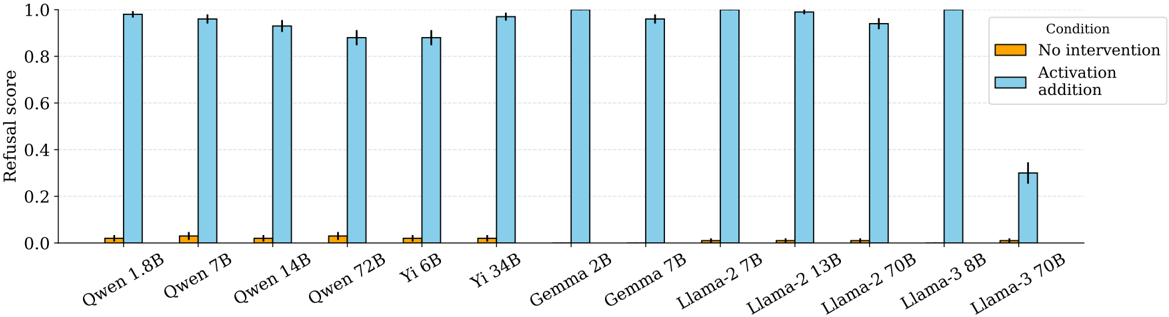
\includegraphics[width=\textwidth,height=0.6\textheight,keepaspectratio]{figures/arditi2024/fig1.png}
\end{column}
\end{columns}

\note{
\begin{itemize}
\item The authors identify the refusal direction in a bunch of different LLMs
\item They can always stop models from refusing by ablating it out
\item Or make them refuse harmless questions by adding it
\end{itemize}
}
\end{frame}
